% L13c lecture companion. Coverage and source hashes are recorded in README.md.
% The style files and Cornell seal are copied unchanged from L13a.
% Figures are the lecture's light TikZ PDFs, copied unchanged into assets/.
% JSON blocks show selected fields from the saved messages. The full messages
% are linked from their slides; omitted metadata is identified explicitly.
\documentclass[aspectratio=169,11pt]{beamer}
\usepackage{vnslides}
\usepackage{fancyvrb}
\renewcommand{\vnlecturecode}{L13c}
\newcommand{\lecturebase}{https://github.com/varnerlab/CHEME-5800-CourseRepository-Fall-2026/blob/main/weeks/week-13/L13c/}
\newcommand{\lecturelink}{\lecturebase CHEME-5800-L13c-Lecture-ModelContextProtocol-Fall-2026.ipynb}
\newcommand{\examplelink}{\lecturebase CHEME-5800-L13c-Example-MCP-NWS-Fall-2026.ipynb}
\newcommand{\speclink}{https://modelcontextprotocol.io/specification/2026-07-28}
\newcommand{\lecturesource}[1]{\note{[Sources]\par
  \href{\lecturelink}{L13c lecture: The Model Context Protocol.}\par
  #1\par[/Sources]}}
\newcommand{\code}[1]{\texttt{#1}}
\newcommand{\jsonfont}{\fontsize{8.2}{10}\selectfont}
\newcommand{\messagepair}[2]{\slidenote{Full messages:}{%
  \href{\lecturebase messages/#1-request.json}{Request}\quad
  \href{\lecturebase messages/#2-response.json}{Response}}}

\title{\texorpdfstring{{\vnheavy L13c}: The Model Context Protocol}{L13c: The Model Context Protocol}}
\subtitle{\texorpdfstring{Language models, tools, and the messages of a tool call\\[3pt]CHEME 5800 Cornell University}{Language models, tools, and the messages of a tool call; CHEME 5800 Cornell University}}
\author{Copyright Jeffrey Varner 2026. All Rights Reserved}

\begin{document}
\special{pdf:minorversion 7}
\vntitlepage

\begin{frame}{Objectives for Today}
  How does a language model application use our computational code?

  \vspace{0.4em}
  {\large\textbf{\ink{Today's concepts}}}
  \vspace{0.2em}
  \begin{itemize}\setlength{\itemsep}{0.5em}
    \item \hilite{Describe the roles in an MCP system}: define the host,
      the client, and the server, and explain how the host controls tool calls.
    \item \hilite{Read the messages of a tool call}: follow the JSON-RPC
      messages that discover a server, list its tools, and call a tool.
    \item \hilite{Identify the trust boundaries of a tool call}: explain
      what the host and the server each check when the model proposes arguments.
  \end{itemize}
  \slidenote{Lecture:}{\href{\lecturelink}{The Model Context Protocol}}
  \lecturesource{Introduction and three Learning Objectives.}
\end{frame}

\begin{frame}{Lecture and Example}
  \textbf{\ink{Lecture:}}
  \href{\lecturelink}{The Model Context Protocol}

  In this lecture, we introduce the Model Context Protocol (MCP), an open
  standard that connects language model applications to tools. We look at the
  roles in an MCP system, the messages of a tool call, and the checks that
  keep a tool call safe.

  \vspace{1.1em}
  \textbf{\ink{Example:}}
  \href{\examplelink}{Build an MCP server for the National Weather Service API}

  In this example, we wrap our software development kit (SDK) for the
  National Weather Service API in an MCP server with two tools. We call the
  tools as a host would, and trigger both kinds of errors.
  \lecturesource{Introduction and the Examples section. Companion example: opening paragraph.}
\end{frame}

\begin{frame}{Language Models and Tools}
  A \hilite{large language model (LLM)} is a neural network that reads and
  writes text. On its own, an LLM cannot look up today's weather or run our
  Julia code.

  \vspace{0.5em}
  An application gives an LLM these abilities through \hilite{tools},
  functions that the application runs when the model asks for them.

  \vspace{0.5em}
  In a \hilite{tool call}:
  \begin{enumerate}\setlength{\itemsep}{0.5em}
    \item The model proposes a tool name and its arguments.
    \item The application runs the tool.
    \item The model writes its answer from the result.
  \end{enumerate}
  \lecturesource{Language Models and Tools: the LLM, tools, and tool-call definitions.}
\end{frame}

\begin{frame}{The Model Context Protocol}
  The \hilite{Model Context Protocol (MCP)} is an open standard that
  connects applications to tools.

  \vspace{0.5em}
  Suppose we have $M$ applications and $N$ tool sources. To connect every
  application to every source, compare:
  \[
    \underbrace{M\times N}_{\text{custom integrations}}
    \qquad\text{or}\qquad
    \underbrace{M+N}_{\text{each side implements MCP once}}.
  \]

  \vspace{0.5em}
  Anthropic released MCP in November 2024. It donated the protocol to the
  Agentic AI Foundation of the Linux Foundation in December 2025.

  \vspace{0.4em}
  We use \href{\speclink}{version \code{2026-07-28} of the MCP specification}.
  \lecturesource{Language Models and Tools: the integration count, history, and specification version.
    Official specification: https://modelcontextprotocol.io/specification/2026-07-28.}
\end{frame}

\begin{frame}{Hosts, Clients, and Servers}
  \centering
  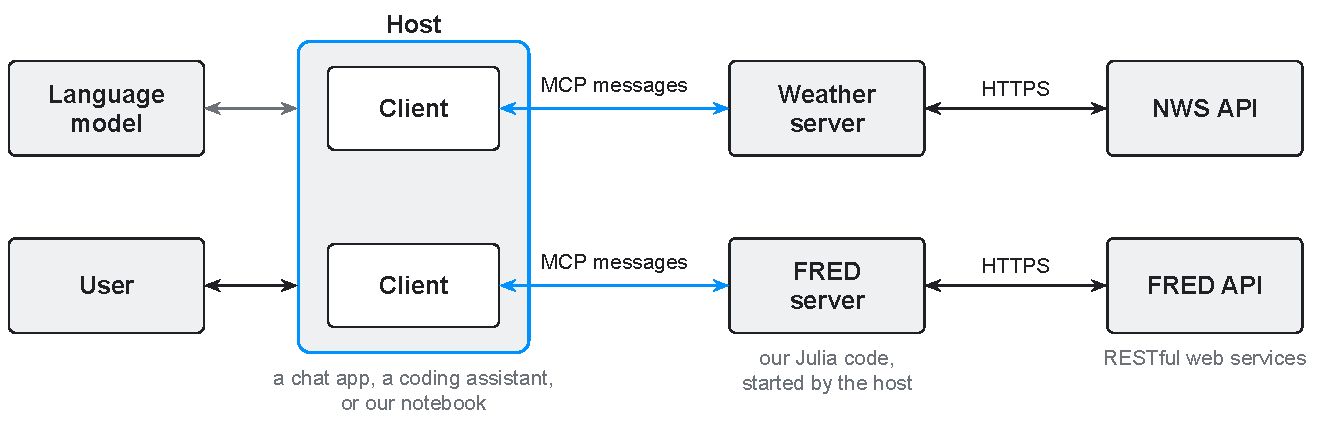
\includegraphics[width=\textwidth,height=0.39\paperheight,keepaspectratio]{assets/Fig-MCP-Architecture.pdf}

  \vspace{0.4em}
  \raggedright
  \begin{itemize}\setlength{\itemsep}{0.35em}
    \item \hilite{Host}: the application the user works with. It manages
      the model, starts our servers, and controls tool calls.
    \item \hilite{Client}: each client runs inside the host and exchanges
      MCP messages with one server.
    \item \hilite{Server}: a server provides tools. Our Julia servers call
      the NWS and FRED APIs over HTTPS.
  \end{itemize}
  \lecturesource{Hosts, Clients, and Servers: the architecture figure and three role definitions.
    Figure: ../figs/Fig-MCP-Architecture/Fig-MCP-Architecture.pdf (light TikZ build).}
\end{frame}

\begin{frame}{Transports}
  A \hilite{transport} carries messages between a client and a server.
  Our servers use \hilite{stdio}:

  \vspace{0.3em}
  \begin{itemize}\setlength{\itemsep}{0.5em}
    \item The host sends requests to the server's \hilite{standard input}.
    \item The host reads replies from the server's \hilite{standard output}.
    \item Each message is one line of JSON text. Standard output carries
      only protocol messages. Julia sends log messages to \hilite{standard error}.
  \end{itemize}

  \vspace{0.5em}
  The protocol also supports \hilite{Streamable HTTP} for servers accessed
  over a network.
  \lecturesource{Hosts, Clients, and Servers: transport, stdio, and Streamable HTTP.
    MCP Messages: one line per message, standard output, and standard error.}
\end{frame}

\begin{frame}{MCP Messages}
  The protocol uses \hilite{JSON-RPC 2.0}, a JSON format for requests
  and responses:

  \vspace{0.5em}
  {\setlength{\tabcolsep}{6pt}%
  \begin{tabular}{>{\raggedright\arraybackslash}p{0.19\textwidth}>{\raggedright\arraybackslash}p{0.73\textwidth}}
    \toprule
    \textbf{Message} & \textbf{Fields and behavior}\\
    \midrule
    Request & Carries \code{jsonrpc} (always \code{"2.0"}), an \code{id},
      the \code{method}, and its \code{params}.\\
    \addlinespace[7pt]
    Response & Repeats the request's \code{id}. Contains either a
      \code{result} or an \code{error}.\\
    \addlinespace[7pt]
    Notification & Has no \code{id} and receives no response.\\
    \bottomrule
  \end{tabular}}

  \vspace{0.7em}
  The \code{id} lets the client match a response to the request that it sent.
  \lecturesource{MCP Messages: request, response, and notification definitions.}
\end{frame}

\begin{frame}[fragile]{Protocol Version \code{2026-07-28}}
  This version is \hilite{stateless}: each request carries its protocol
  version, client identity, and capabilities in \code{params.\_meta}.

  \vspace{0.5em}
  \begin{columns}[T,onlytextwidth]
    \begin{column}{0.58\textwidth}
      \textbf{\ink{The \code{\_meta} object of our requests}}
\begin{Verbatim}[fontsize=\jsonfont]
{
  "io.modelcontextprotocol/protocolVersion":
    "2026-07-28",
  "io.modelcontextprotocol/clientInfo": {
    "name": "cheme-5800-notebook",
    "version": "1.0.0"
  },
  "io.modelcontextprotocol/clientCapabilities": {}
}
\end{Verbatim}
    \end{column}
    \begin{column}{0.38\textwidth}
      The server checks the version on every request.

      \vspace{0.6em}
      Our servers reject the older \code{initialize} handshake with error
      \code{-32022} because it lacks this metadata.
    \end{column}
  \end{columns}
  \lecturesource{MCP Messages: stateless requests and rejection of the older initialize handshake.
    Metadata copied from messages/1-discover-request.json.}
\end{frame}

\begin{frame}{JSON-RPC Errors}
  An \code{error} contains a numeric \code{code} and a \code{message}.
  Our servers use six codes:

  \vspace{0.4em}
  {\small\setlength{\tabcolsep}{6pt}%
  \begin{tabular}{>{\raggedright\arraybackslash}p{0.16\textwidth}>{\raggedright\arraybackslash}p{0.76\textwidth}}
    \toprule
    \textbf{Code} & \textbf{Meaning}\\
    \midrule
    \code{-32700} & Parse error: the message is not valid JSON.\\
    \addlinespace[5pt]
    \code{-32600} & Invalid request: the message is not a JSON-RPC 2.0 request,
      e.g., its \code{jsonrpc} field is missing.\\
    \addlinespace[5pt]
    \code{-32601} & Method not found: the server has no method with this name.\\
    \addlinespace[5pt]
    \code{-32602} & Invalid params, e.g., the request names an unavailable tool.\\
    \addlinespace[5pt]
    \code{-32603} & Internal error: the server failed while processing the request.\\
    \addlinespace[5pt]
    \code{-32022} & Unsupported protocol version.\\
    \bottomrule
  \end{tabular}}
  \lecturesource{MCP Messages: the six-code error table.}
\end{frame}

\begin{frame}[fragile]{Discover a Server}
  A \code{server/discover} request asks which protocol versions and
  capabilities the server supports.

  \vspace{0.5em}
  \begin{columns}[T,onlytextwidth]
    \begin{column}{0.52\textwidth}
      \textbf{\ink{Selected fields from \code{result}}}
\begin{Verbatim}[fontsize=\jsonfont]
{
  "supportedVersions": [
    "2026-07-28"
  ],
  "capabilities": {
    "tools": {}
  },
  "ttlMs": 3600000
}
\end{Verbatim}
    \end{column}
    \begin{column}{0.44\textwidth}
      Our server advertises tools and supplies \code{instructions} for
      the model.

      \vspace{0.5em}
      Its identity appears in \code{\_meta}.

      \vspace{0.5em}
      The \code{ttlMs} value permits reuse of this response for one hour.
    \end{column}
  \end{columns}
  \messagepair{1-discover}{1-discover}
  \lecturesource{MCP Messages / Discover a Server.
    Saved request and response: messages/1-discover-request.json and messages/1-discover-response.json.}
\end{frame}

\begin{frame}{List the Tools}
  A \code{tools/list} request returns each tool's \code{name},
  \code{description}, and \code{inputSchema}.

  \vspace{0.5em}
  {\small\setlength{\tabcolsep}{6pt}%
  \begin{tabular}{>{\raggedright\arraybackslash}p{0.36\textwidth}>{\raggedright\arraybackslash}p{0.56\textwidth}}
    \toprule
    \textbf{Tool} & \textbf{What it does}\\
    \midrule
    \code{get\_hourly\_forecast} & Gets temperature, wind, and a short forecast
      for each hour at a location in the United States.\\
    \addlinespace[7pt]
    \code{get\_location} & Finds the nearest city, the state, and the NWS
      forecast office of a location in the United States.\\
    \bottomrule
  \end{tabular}}

  \vspace{0.7em}
  The model uses the description to choose a tool. The input schema defines
  the arguments that the tool accepts.
  \messagepair{2-list}{2-list}
  \lecturesource{MCP Messages / List the Tools. Tool descriptions from messages/2-list-response.json.
    Companion example: Task 2.}
\end{frame}

\begin{frame}[fragile]{The Input Schema}
  The input schema uses \hilite{JSON Schema} to define arguments, their
  types, and which are required.

  \vspace{0.4em}
  \begin{columns}[T,onlytextwidth]
    \begin{column}{0.57\textwidth}
      \textbf{\ink{Selected schema fields}}
\begin{Verbatim}[fontsize=\jsonfont]
{
  "type": "object",
  "properties": {
    "latitude": {"type": "number"},
    "longitude": {"type": "number"},
    "hours": {
      "type": "integer",
      "minimum": 1,
      "maximum": 48
    }
  },
  "required": ["latitude", "longitude"]
}
\end{Verbatim}
    \end{column}
    \begin{column}{0.39\textwidth}
      For \code{get\_hourly\_forecast}, \code{latitude} and
      \code{longitude} are required numbers.

      \vspace{0.6em}
      The optional \code{hours} argument is an integer from \code{1} to
      \code{48}.
    \end{column}
  \end{columns}
  \lecturesource{MCP Messages / List the Tools: JSON Schema and the forecast arguments.
    Excerpt: messages/2-list-response.json. Descriptions and latitude/longitude limits omitted from the displayed schema.}
\end{frame}

\begin{frame}[fragile]{Call a Tool}
  A \code{tools/call} request gives the tool's name and arguments.
  Here, we request a one-hour forecast for Ithaca, NY.

  \vspace{0.5em}
  \begin{columns}[T,onlytextwidth]
    \begin{column}{0.55\textwidth}
      \textbf{\ink{Request fields, with metadata omitted}}
\begin{Verbatim}[fontsize=\jsonfont]
{
  "jsonrpc": "2.0",
  "id": 3,
  "method": "tools/call",
  "params": {
    "name": "get_hourly_forecast",
    "arguments": {
      "latitude": 42.443961,
      "longitude": -76.501881,
      "hours": 1
    }
  }
}
\end{Verbatim}
    \end{column}
    \begin{column}{0.41\textwidth}
      The \code{name} selects a tool from the server's list.

      \vspace{0.6em}
      The \code{arguments} object supplies values that match its schema.

      \vspace{0.6em}
      The response repeats \code{id: 3}.
    \end{column}
  \end{columns}
  \messagepair{3-call}{3-call}
  \lecturesource{MCP Messages / Call a Tool.
    Excerpt: messages/3-call-request.json, with params._meta omitted for projection.}
\end{frame}

\begin{frame}[fragile]{The Tool Result}
  A successful call returns a \code{result} with \code{isError} set
  to \code{false}.

  \vspace{0.5em}
  \begin{columns}[T,onlytextwidth]
    \begin{column}{0.54\textwidth}
      \textbf{\ink{One period in \code{structuredContent}}}
\begin{Verbatim}[fontsize=\jsonfont]
{
  "short_forecast": "Light Rain",
  "start_time":
    "2026-11-12T22:00:00-05:00",
  "temperature": 37,
  "temperature_unit": "F",
  "wind_direction": "N",
  "wind_speed": "7 mph"
}
\end{Verbatim}
    \end{column}
    \begin{column}{0.42\textwidth}
      The \code{content} array provides text for the model.

      \vspace{0.6em}
      The \code{structuredContent} field provides the same result as JSON
      data for a program.

      \vspace{0.6em}
      This is the saved November 12, 2026 response.
    \end{column}
  \end{columns}
  \messagepair{3-call}{3-call}
  \lecturesource{MCP Messages / Call a Tool: content, structuredContent, and isError.
    Forecast period copied from messages/3-call-response.json. It is a saved example, not a live forecast.}
\end{frame}

\begin{frame}{One Tool Call}
  \centering
  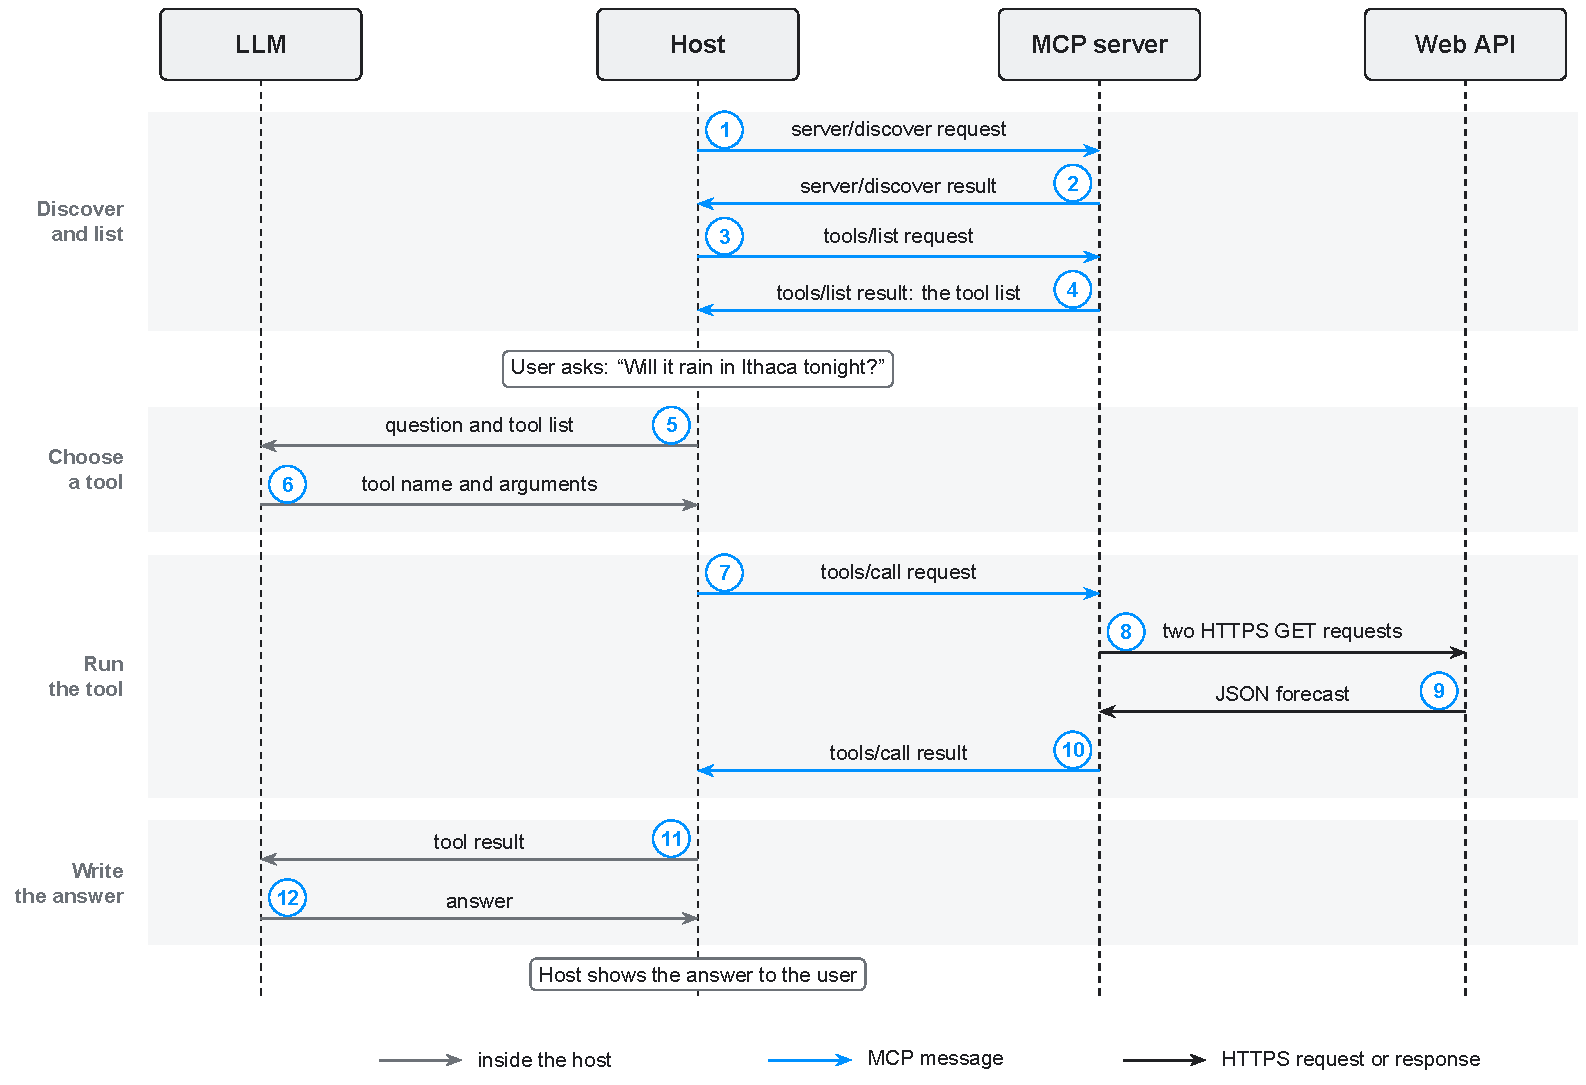
\includegraphics[width=\textwidth,height=0.65\paperheight,keepaspectratio]{assets/Fig-MCP-ToolCall.pdf}

  \vspace{0.3em}
  \raggedright
  Gray arrows stay within the host, blue arrows carry MCP messages, and dark
  arrows carry HTTPS requests and responses. Our weather server makes two
  API requests.
  \lecturesource{MCP Messages / Call a Tool: the sequence figure and its caption.
    Figure: ../figs/Fig-MCP-ToolCall/Fig-MCP-ToolCall.pdf (light TikZ build).}
\end{frame}

\begin{frame}[fragile]{Two Kinds of Errors}
  \begin{columns}[T,onlytextwidth]
    \begin{column}{0.48\textwidth}
      \textbf{\ink{Protocol error}}

      The request names an unavailable \code{get\_snowfall} tool.
\begin{Verbatim}[fontsize=\jsonfont]
{
  "jsonrpc": "2.0", "id": 4,
  "error": {
    "code": -32602,
    "message":
      "Unknown tool: get_snowfall"
  }
}
\end{Verbatim}
      The response has an \code{error} and no \code{result}. Protocol errors
      usually indicate a host or server bug.
    \end{column}
    \begin{column}{0.48\textwidth}
      \textbf{\ink{Tool execution error}}

      The Paris forecast request reaches the NWS API, which does not cover
      that location.
\begin{Verbatim}[fontsize=\jsonfont]
{
  "jsonrpc": "2.0", "id": 5,
  "result": {
    "isError": true
  }
}
\end{Verbatim}
      These selected fields show a normal \code{result}. Its error text
      explains the failure to the model, which can choose different arguments.
    \end{column}
  \end{columns}
  \slidenote{Full messages:}{%
    \href{\lecturebase messages/4-unknown-tool-request.json}{Unknown-tool request}\quad
    \href{\lecturebase messages/4-unknown-tool-response.json}{Response}\quad
    \href{\lecturebase messages/5-paris-request.json}{Paris request}\quad
    \href{\lecturebase messages/5-paris-response.json}{Response}}
  \lecturesource{MCP Messages / Two Kinds of Errors.
    Protocol response: messages/4-unknown-tool-response.json.
    Tool execution response excerpt: messages/5-paris-response.json, with metadata and content omitted.}
\end{frame}

\begin{frame}{The Server Loop}
  \textbf{\ink{Initialize:}} Given a set of tools $\mathcal{T}$, each with
  a name, a description, an input schema, and a \hilite{handler} (the
  function that runs the tool), and protocol version $v\gets$ \code{2026-07-28}.

  \vspace{0.4em}
  While standard input is open, read the next nonblank line $\ell$ and parse
  it into a message $m$. Choose a response $r$ from the first matching rule:

  \vspace{0.3em}
  {\small\setlength{\tabcolsep}{6pt}%
  \begin{tabular}{>{\raggedright\arraybackslash}p{0.57\textwidth}>{\raggedright\arraybackslash}p{0.35\textwidth}}
    \toprule
    \textbf{Message check} & \textbf{Response $r$}\\
    \midrule
    $\ell$ is not valid JSON. & Parse error, \code{-32700}.\\
    \addlinespace[5pt]
    $m$ is not a JSON-RPC 2.0 message. & Invalid request, \code{-32600}.\\
    \addlinespace[5pt]
    $m$ has no \code{id}. & $\texttt{nothing}$ (notification).\\
    \addlinespace[5pt]
    The \code{\_meta} object does not name $v$. & Unsupported version, \code{-32022}.\\
    \bottomrule
  \end{tabular}}

  \vspace{0.4em}
  If these checks pass, route the request by its method.
  \lecturesource{MCP Messages / The Server Loop: Initialize, read/parse, and the first four response rules.}
\end{frame}

\begin{frame}{The Server Loop: Routing}
  After the message checks, choose the response $r$ by the request's method:

  \vspace{0.4em}
  {\small\setlength{\tabcolsep}{6pt}%
  \begin{tabular}{>{\raggedright\arraybackslash}p{0.39\textwidth}>{\raggedright\arraybackslash}p{0.53\textwidth}}
    \toprule
    \textbf{Method or condition} & \textbf{Response $r$}\\
    \midrule
    \code{server/discover} & Versions, capabilities, and server identity.\\
    \addlinespace[5pt]
    \code{tools/list} & Each tool's name, description, and input schema.\\
    \addlinespace[5pt]
    \code{tools/call}, known tool & Run the handler. Set \code{isError: true}
      in its result if it fails.\\
    \addlinespace[5pt]
    \code{tools/call}, unknown tool & Invalid params, \code{-32602}.\\
    \addlinespace[5pt]
    Any other method & Method not found, \code{-32601}.\\
    \bottomrule
  \end{tabular}}

  \vspace{0.4em}
  Write any response $r\neq\texttt{nothing}$ as one line of JSON to standard
  output. Stop when the client closes standard input.
  \slidenote{Code:}{\href{\lecturebase src/Server.jl}{The message processor and server loop}}
  \lecturesource{MCP Messages / The Server Loop: the method-routing rules, write step, Output, and code links.}
\end{frame}

\begin{frame}{Trust and Security}
  The weather example crosses three \hilite{trust boundaries}:

  \vspace{0.5em}
  \begin{itemize}\setlength{\itemsep}{0.7em}
    \item \hilite{Model $\rightarrow$ host}: the model proposes a tool and
      arguments. The host decides whether the call is permitted and asks for
      user approval when needed.
    \item \hilite{Host $\rightarrow$ server}: our stdio servers run locally
      with the user's permissions. Install only servers whose code you trust.
    \item \hilite{Server $\rightarrow$ API}: the server validates tool
      arguments before making an API request. It keeps API keys out of MCP messages.
  \end{itemize}
  \lecturesource{Trust and Security: the three trust boundaries.}
\end{frame}

\begin{frame}{Prompt Injection and User Approval}
  \hilite{Prompt injection} occurs when text returned by a server tries
  to redirect the model toward actions the user did not request.

  \vspace{1.0em}
  Our tools read public data. Tools that change data, such as placing an
  order, should require user approval for each call.
  \lecturesource{Trust and Security: prompt injection and approval for tools that change data.}
\end{frame}

\begin{frame}{Example: An MCP Server for the NWS API}
  In this example, we wrap our NWS SDK in a server with two tools.
  We play the host and make the calls that a host would make for its model:

  \vspace{0.5em}
  \begin{enumerate}\setlength{\itemsep}{0.6em}
    \item \hilite{Start and discover the server}: start the Julia server
      as a subprocess and read its protocol version, capabilities, and identity.
    \item \hilite{List the tools}: read the two tool descriptions and
      the input schema of \code{get\_hourly\_forecast}.
    \item \hilite{Call the tools}: find Ithaca's forecast office and put
      its hourly forecast into a table. Trigger an unknown-tool error and a
      forecast failure for Paris, France.
  \end{enumerate}

  \vspace{0.5em}
  We close the server's standard input when we finish. The server exits.
  \slidenote{Example:}{\href{\examplelink}{Build an MCP server for the National Weather Service API}}
  \lecturesource{Examples. Companion example: Tasks 1--3 and Close the Connection.}
\end{frame}

\begin{frame}{Summary}
  We introduced the Model Context Protocol, the messages of a tool call, and
  the checks that keep a tool call safe.

  \vspace{0.4em}
  {\large\textbf{\ink{Key takeaways}}}
  \vspace{0.2em}
  \begin{itemize}\setlength{\itemsep}{0.4em}
    \item \textbf{\ink{Hosts, clients, and servers.}} We separated their
      roles. The host runs a client for each server, and every tool call
      passes through the host.
    \item \textbf{\ink{Discover, list, and call.}} We followed JSON-RPC
      requests that name the protocol version. A wrong request gets a protocol
      error. A tool that fails returns a result with its error flag set.
    \item \textbf{\ink{Trust boundaries.}} We identified what each side
      checks. The host permits the call, and the server validates its arguments
      and keeps API keys out of MCP messages.
  \end{itemize}

  \vspace{0.4em}
  Any language model application that supports this protocol version can
  use our own computational code.
  \lecturesource{Summary: opening sentence, three key takeaways, and closing sentence.}
\end{frame}

\end{document}
